\section{Versuchsaufbau und Messgeräte}
Unser Versuch findet aufgrund der nötigen Kühlung mit flüssigem Stickstoff in einem Kryostaten statt. Gleichzeitig ist eine Heizwicklung direkt am Probenträger angebracht, um auch höhere Temperaturbereiche vermessen zu können. Der gesamte Kryostat wird weiterhin unter Vakuum betrieben, für das eine Diffusionspumpe verwendet wird. Im Falle von konventionellen Hall-Effekt-Vermessungen wird von einer quaderförmigen Probengeometrie ausgegangen, um Widerstände quer und längs der Probe wohl definiert bestimmen zu können. In unserem Versuchsaufbau kommt dagegen die sogenannte Van-der-Pauw-Methode zum Einsatz. Bei dieser wird eine undefiniert geformte Germaniumprobe in konstanter Dicke auf eine Trägerplatte aufgedampft. Hierdurch lässt sich eine nahezu planparallele Form der Probe darstellen. An die Ge-Probe werden vier Anschlüsse A, B, C und D angebracht, wobei zwischen zwei Anschlüssen der Messstrom fließen wird und an den anderen beiden der Spannungsabfall gemessen. Um zwischen den Messanschlüssen umschalten zu können, sind die jeweiligen Anschlussleitungen mit einer Umschaltbox verbunden, sodass jegliche Strom- und Spannungskontaktkombinationen vermessen werden können (siehe Abbildung \ref{aufbau}). 

\begin{figure}[htbp]  
     \usetikzlibrary{shapes,arrows}
\tikzstyle{block} = [draw, fill=blue!20, rectangle, 
    minimum height=1em, minimum width=2em]
\tikzstyle{circle} = [draw, fill=blue!20, ellipse, 
    minimum height=1.5em, minimum width=1.5em]
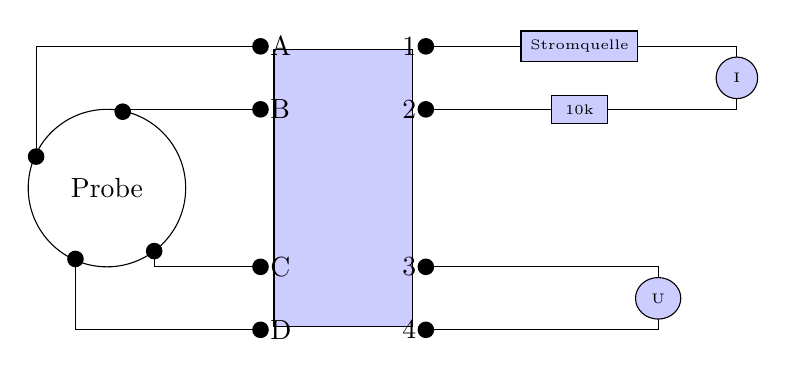
\begin{tikzpicture}
 \coordinate (L) at (-5,0);
\coordinate (R1) at (2,-1.4);
\coordinate (R2) at (3,1.4);
\coordinate (M1) at (1, 1.0);
\coordinate (M2) at (1, 1.8);


 \coordinate (A1) at (-5.9,0.4);
\coordinate (B1) at (-4.8,0.97);
\coordinate (C1) at (-4.4,-0.8);
\coordinate (D1) at (-5.4,-0.9);

\coordinate (A2) at (-3.05,1.8);
\coordinate (B2) at (-3.05,1.0);
\coordinate (C2) at (-3.05,-1.0);
\coordinate (D2) at (-3.05,-1.8);

\coordinate (A3) at (-0.95,1.8);
\coordinate (B3) at (-0.95,1.0);
\coordinate (C3) at (-0.95,-1.0);
\coordinate (D3) at (-0.95,-1.8);
\draw (L) circle [radius=1];
\node (probe) at (L) {Probe};

\fill[black] (A1) circle (3pt);
\fill[black] (B1) circle (3pt);
\fill[black] (C1) circle (3pt);
\fill[black] (D1) circle (3pt);

\node[block, minimum height=10em, minimum width=5em] at (-2,0) {};
\fill[black] (A2) circle (3pt);
\fill[black] (B2) circle (3pt);
\fill[black] (C2) circle (3pt);
\fill[black] (D2) circle (3pt);
\draw (A1) |- (A2);
\draw (B1) |- (B2);
\draw (C1) |- (C2);
\draw (D1) |- (D2);
\fill[black] (A3) circle (3pt);
\fill[black] (B3) circle (3pt);
\fill[black] (C3) circle (3pt);
\fill[black] (D3) circle (3pt);
\draw (A2) node[right] {A};
\draw (B2) node[right] {B};
\draw (C2) node[right] {C};
\draw (D2) node[right] {D};
\draw (A3) node[left] {1};
\draw (B3) node[left] {2};
\draw (C3) node[left] {3};
\draw (D3) node[left] {4};

\draw (D3) -| (R1);
\draw (C3) -| (R1);
\node[circle] at (R1) {\tiny U};

\draw (B3) -- (M1);
\draw (M1) -| (R2);
\draw (A3) -- (M2);
\draw (M2) -| (R2);
\node[block] at (M1) {\tiny 10k};
\node[circle] at (R2) {\tiny I};
\node[block] at (M2) {\tiny Stromquelle};
\end{tikzpicture}
  \caption{Schematischer Versuchsaufbau mit Strom- und Spannungsmessung an der Probe}
  \label{aufbau}
\end{figure}

Um nun das für die Vermessung des Hall-Effekts benötigte Magnetfeld anlegen zu können, befindet sich eine Spule am Kryostat. Aufgrund des magnetoresistiven Effekts treten bei der Vermessung des Hall-Effekts unerwüschte Widerstandsänderungen auf, welche unsere Messung verfälschen. Um diese zu minimieren legen wir daher unser Magnetfeld einmal in positiver und einmal in negativer Richtung an, anstatt den Fall mit Magnetfeld zu dem ohne zu vergleichen. Anschaulich gesprochen ändern wir hierfür die Stromrichtung in der Spule. Dafür sind die Spulenanschlüsse mit einem Schalter gekoppelt, über den sich die Stromrichtung umdrehen lässt. Durch den angelegten Strom und die gemessenen Potentialdifferenz lässt sich folgender Widerstand definieren:

\begin{align}
R_{AB,CD}= \frac{V_D -V_C}{I_{AB}}
\end{align}

Aus verschiedenen Kombinationen der Anschlüsse für den angelegten Stroms und die gemessene Spannung lässt sich der spezifische Widerstand der Probe herleiten:

\begin{align}
\rho = \frac{\pi d}{\log{2}}\left(\frac{R_{AB,CD}+R_{BC,DA}}{2}\right)f\left(\frac{R_{AB,CD}}{R_{BC,DA}}\right)
\end{align}

Die Funktion $f$ stellt dabei einen nicht-analytischen Korrekturfaktor dar, welchen wir aus einer in der Anleitung gegebenen Grafik ablesen können. 

Der Hall-Koeffizient lässt sich ebenfalls mit der van-der-Pauw-Methode bestimmen und ergibt sich zu:

\begin{align}
R_H=\frac{1}{en}=\frac{d}{B}\Delta R_{BD,AC}
\end{align}

Für die Temperaturmessung haben wir weiterhin ein Thermospannungselement im Kryostaten hängen. Dieses misst die über eine Temperaturdifferenz abfallende Spannung. Da die Zimmertemperatur als Referenztemperatur zu ungenau ist, verwenden wir ein Becherglas mit Eiswasser als Referenz. Die im Becherglas vorliegende Temperatur beträgt aufgrund des Phasenübergangs exakt $0^{\circ}C$, sodass wir die gemessene Thermospannung in Temperatur umrechnen können. Die entsprechende Eichtabelle findet sich in der Anleitung des Versuchs.

Während die Abkühlung des Versuchsaufbaus mithilfe von flüssigem Stickstoff realisiert wird, verwenden wir für den höheren Temperaturbereich einen Heizdraht, welcher mit maximal $5V$ betrieben wird und die Probe langsam aufheizt. 
